% Options for packages loaded elsewhere
\PassOptionsToPackage{unicode}{hyperref}
\PassOptionsToPackage{hyphens}{url}
%
\documentclass[
]{book}
\usepackage{lmodern}
\usepackage{amssymb,amsmath}
\usepackage{ifxetex,ifluatex}
\ifnum 0\ifxetex 1\fi\ifluatex 1\fi=0 % if pdftex
  \usepackage[T1]{fontenc}
  \usepackage[utf8]{inputenc}
  \usepackage{textcomp} % provide euro and other symbols
\else % if luatex or xetex
  \usepackage{unicode-math}
  \defaultfontfeatures{Scale=MatchLowercase}
  \defaultfontfeatures[\rmfamily]{Ligatures=TeX,Scale=1}
\fi
% Use upquote if available, for straight quotes in verbatim environments
\IfFileExists{upquote.sty}{\usepackage{upquote}}{}
\IfFileExists{microtype.sty}{% use microtype if available
  \usepackage[]{microtype}
  \UseMicrotypeSet[protrusion]{basicmath} % disable protrusion for tt fonts
}{}
\makeatletter
\@ifundefined{KOMAClassName}{% if non-KOMA class
  \IfFileExists{parskip.sty}{%
    \usepackage{parskip}
  }{% else
    \setlength{\parindent}{0pt}
    \setlength{\parskip}{6pt plus 2pt minus 1pt}}
}{% if KOMA class
  \KOMAoptions{parskip=half}}
\makeatother
\usepackage{xcolor}
\IfFileExists{xurl.sty}{\usepackage{xurl}}{} % add URL line breaks if available
\IfFileExists{bookmark.sty}{\usepackage{bookmark}}{\usepackage{hyperref}}
\hypersetup{
  pdftitle={Exploratory Data Analysis},
  pdfauthor={Sebnem Er},
  hidelinks,
  pdfcreator={LaTeX via pandoc}}
\urlstyle{same} % disable monospaced font for URLs
\usepackage{color}
\usepackage{fancyvrb}
\newcommand{\VerbBar}{|}
\newcommand{\VERB}{\Verb[commandchars=\\\{\}]}
\DefineVerbatimEnvironment{Highlighting}{Verbatim}{commandchars=\\\{\}}
% Add ',fontsize=\small' for more characters per line
\usepackage{framed}
\definecolor{shadecolor}{RGB}{248,248,248}
\newenvironment{Shaded}{\begin{snugshade}}{\end{snugshade}}
\newcommand{\AlertTok}[1]{\textcolor[rgb]{0.94,0.16,0.16}{#1}}
\newcommand{\AnnotationTok}[1]{\textcolor[rgb]{0.56,0.35,0.01}{\textbf{\textit{#1}}}}
\newcommand{\AttributeTok}[1]{\textcolor[rgb]{0.77,0.63,0.00}{#1}}
\newcommand{\BaseNTok}[1]{\textcolor[rgb]{0.00,0.00,0.81}{#1}}
\newcommand{\BuiltInTok}[1]{#1}
\newcommand{\CharTok}[1]{\textcolor[rgb]{0.31,0.60,0.02}{#1}}
\newcommand{\CommentTok}[1]{\textcolor[rgb]{0.56,0.35,0.01}{\textit{#1}}}
\newcommand{\CommentVarTok}[1]{\textcolor[rgb]{0.56,0.35,0.01}{\textbf{\textit{#1}}}}
\newcommand{\ConstantTok}[1]{\textcolor[rgb]{0.00,0.00,0.00}{#1}}
\newcommand{\ControlFlowTok}[1]{\textcolor[rgb]{0.13,0.29,0.53}{\textbf{#1}}}
\newcommand{\DataTypeTok}[1]{\textcolor[rgb]{0.13,0.29,0.53}{#1}}
\newcommand{\DecValTok}[1]{\textcolor[rgb]{0.00,0.00,0.81}{#1}}
\newcommand{\DocumentationTok}[1]{\textcolor[rgb]{0.56,0.35,0.01}{\textbf{\textit{#1}}}}
\newcommand{\ErrorTok}[1]{\textcolor[rgb]{0.64,0.00,0.00}{\textbf{#1}}}
\newcommand{\ExtensionTok}[1]{#1}
\newcommand{\FloatTok}[1]{\textcolor[rgb]{0.00,0.00,0.81}{#1}}
\newcommand{\FunctionTok}[1]{\textcolor[rgb]{0.00,0.00,0.00}{#1}}
\newcommand{\ImportTok}[1]{#1}
\newcommand{\InformationTok}[1]{\textcolor[rgb]{0.56,0.35,0.01}{\textbf{\textit{#1}}}}
\newcommand{\KeywordTok}[1]{\textcolor[rgb]{0.13,0.29,0.53}{\textbf{#1}}}
\newcommand{\NormalTok}[1]{#1}
\newcommand{\OperatorTok}[1]{\textcolor[rgb]{0.81,0.36,0.00}{\textbf{#1}}}
\newcommand{\OtherTok}[1]{\textcolor[rgb]{0.56,0.35,0.01}{#1}}
\newcommand{\PreprocessorTok}[1]{\textcolor[rgb]{0.56,0.35,0.01}{\textit{#1}}}
\newcommand{\RegionMarkerTok}[1]{#1}
\newcommand{\SpecialCharTok}[1]{\textcolor[rgb]{0.00,0.00,0.00}{#1}}
\newcommand{\SpecialStringTok}[1]{\textcolor[rgb]{0.31,0.60,0.02}{#1}}
\newcommand{\StringTok}[1]{\textcolor[rgb]{0.31,0.60,0.02}{#1}}
\newcommand{\VariableTok}[1]{\textcolor[rgb]{0.00,0.00,0.00}{#1}}
\newcommand{\VerbatimStringTok}[1]{\textcolor[rgb]{0.31,0.60,0.02}{#1}}
\newcommand{\WarningTok}[1]{\textcolor[rgb]{0.56,0.35,0.01}{\textbf{\textit{#1}}}}
\usepackage{longtable,booktabs}
% Correct order of tables after \paragraph or \subparagraph
\usepackage{etoolbox}
\makeatletter
\patchcmd\longtable{\par}{\if@noskipsec\mbox{}\fi\par}{}{}
\makeatother
% Allow footnotes in longtable head/foot
\IfFileExists{footnotehyper.sty}{\usepackage{footnotehyper}}{\usepackage{footnote}}
\makesavenoteenv{longtable}
\usepackage{graphicx,grffile}
\makeatletter
\def\maxwidth{\ifdim\Gin@nat@width>\linewidth\linewidth\else\Gin@nat@width\fi}
\def\maxheight{\ifdim\Gin@nat@height>\textheight\textheight\else\Gin@nat@height\fi}
\makeatother
% Scale images if necessary, so that they will not overflow the page
% margins by default, and it is still possible to overwrite the defaults
% using explicit options in \includegraphics[width, height, ...]{}
\setkeys{Gin}{width=\maxwidth,height=\maxheight,keepaspectratio}
% Set default figure placement to htbp
\makeatletter
\def\fps@figure{htbp}
\makeatother
\setlength{\emergencystretch}{3em} % prevent overfull lines
\providecommand{\tightlist}{%
  \setlength{\itemsep}{0pt}\setlength{\parskip}{0pt}}
\setcounter{secnumdepth}{5}
\usepackage{booktabs}
\usepackage{amsthm}
\makeatletter
\def\thm@space@setup{%
  \thm@preskip=8pt plus 2pt minus 4pt
  \thm@postskip=\thm@preskip
}
\makeatother
\usepackage[]{natbib}
\bibliographystyle{apalike}

\title{Exploratory Data Analysis}
\author{Sebnem Er}
\date{2021-03-04}

\begin{document}
\maketitle

{
\setcounter{tocdepth}{1}
\tableofcontents
}
\hypertarget{introduction}{%
\chapter{Introduction}\label{introduction}}

As part of the MSc specializing in Data Science, this course aims to introduce the essential techniques for performing exploratory data analysis. These techniques are typically applied before formal modeling commences and allow the researcher to discover patterns, spot anomalies, test hypotheses and check assumptions with the help of summary statistics and graphical representations. Different types of data will be described and the appropriate exploratory data analysis techniques for each data type will be introduced. The course will distinguish between univariate non-graphical, multivariate non-graphical, univariate graphical, and multivariate graphical techniques. Special attention will focus on the visualization of large data dets using appropriate software. Some of the topics to be covered include:

\begin{enumerate}
\def\labelenumi{\arabic{enumi})}
\tightlist
\item
  Plotting the raw data (such as data traces, histograms, bihistograms, probability plots, lag plots, block plots, and Youden plots).
\item
  Plotting simple statistics such as mean plots, standard deviation plots, box plots, and main effects plots of the raw data.
\item
  Positioning such plots so as to maximize our natural pattern-recognition abilities, such as using multiple plots per page.
\item
  Plotting geocoded data and creating dashboards
\item
  Dimensionality reduction and clustering of similar observations
\end{enumerate}

Resources

There are some really good free online textbooks by well known and respected teachers in this area -- most of the material we need can be based on these three sources:

\begin{enumerate}
\def\labelenumi{\arabic{enumi}.}
\item
  Exploratory Data Analysis with R (Roger Peng = RP): \url{https://bookdown.org/rdpeng/exdata/}
\item
  STA545: Data wrangling, exploration, and analysis with R (Jenny Bryan = JB): \url{https://stat545.com/index.html}
\item
  R for data science (Hadley Wickham = HW): \url{https://r4ds.had.co.nz/}
\end{enumerate}

\hypertarget{eda-lecture-1-2-r-examples}{%
\chapter{EDA Lecture 1-2 R Examples}\label{eda-lecture-1-2-r-examples}}

\hypertarget{example-2---gapminder}{%
\section{Example 2 - Gapminder}\label{example-2---gapminder}}

\begin{Shaded}
\begin{Highlighting}[]
\CommentTok{#install.packages("gapminder")}
\KeywordTok{library}\NormalTok{(gapminder)}
\NormalTok{gapminder}
\end{Highlighting}
\end{Shaded}

\begin{verbatim}
## # A tibble: 1,704 x 6
##    country     continent  year lifeExp      pop gdpPercap
##    <fct>       <fct>     <int>   <dbl>    <int>     <dbl>
##  1 Afghanistan Asia       1952    28.8  8425333      779.
##  2 Afghanistan Asia       1957    30.3  9240934      821.
##  3 Afghanistan Asia       1962    32.0 10267083      853.
##  4 Afghanistan Asia       1967    34.0 11537966      836.
##  5 Afghanistan Asia       1972    36.1 13079460      740.
##  6 Afghanistan Asia       1977    38.4 14880372      786.
##  7 Afghanistan Asia       1982    39.9 12881816      978.
##  8 Afghanistan Asia       1987    40.8 13867957      852.
##  9 Afghanistan Asia       1992    41.7 16317921      649.
## 10 Afghanistan Asia       1997    41.8 22227415      635.
## # ... with 1,694 more rows
\end{verbatim}

\pagebreak

\hypertarget{frequency-distribution}{%
\section{Frequency Distribution}\label{frequency-distribution}}

\begin{Shaded}
\begin{Highlighting}[]
\KeywordTok{library}\NormalTok{(ggplot2)}
\KeywordTok{table}\NormalTok{(gapminder}\OperatorTok{$}\NormalTok{continent)}
\end{Highlighting}
\end{Shaded}

\begin{verbatim}
## 
##   Africa Americas     Asia   Europe  Oceania 
##      624      300      396      360       24
\end{verbatim}

\hypertarget{bar-plot}{%
\section{Bar Plot}\label{bar-plot}}

\begin{Shaded}
\begin{Highlighting}[]
\KeywordTok{library}\NormalTok{(ggplot2)}
\NormalTok{plot1 <-}\StringTok{ }\KeywordTok{ggplot}\NormalTok{(gapminder, }\KeywordTok{aes}\NormalTok{(}\DataTypeTok{x=}\NormalTok{continent)) }\OperatorTok{+}\StringTok{ }\KeywordTok{geom_bar}\NormalTok{()}
\NormalTok{plot1}
\end{Highlighting}
\end{Shaded}

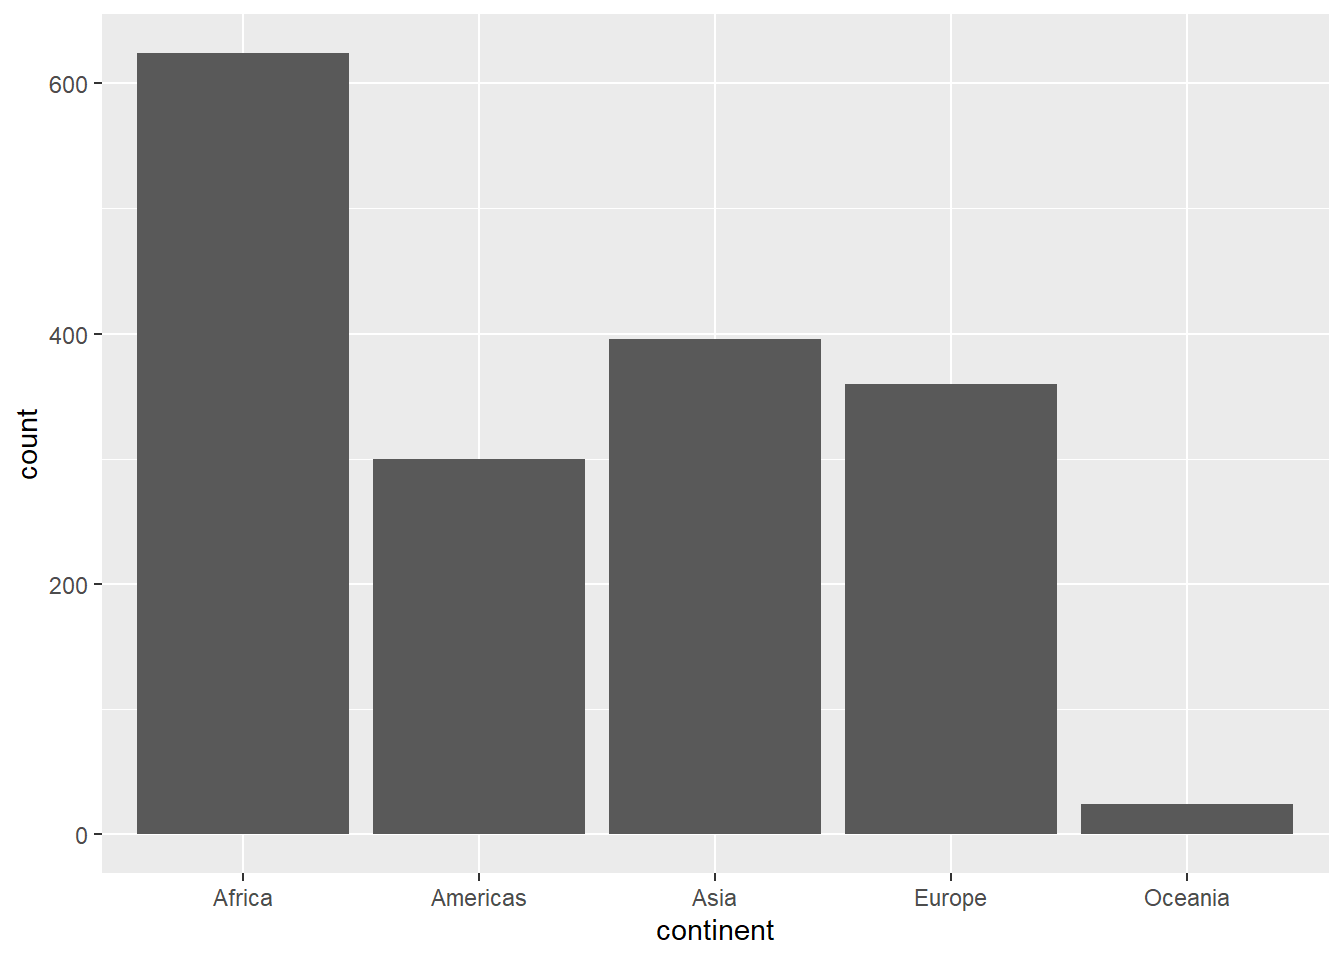
\includegraphics{bookdown-demo_files/figure-latex/unnamed-chunk-4-1.pdf}

\hypertarget{pie-chart}{%
\section{Pie Chart}\label{pie-chart}}

\begin{Shaded}
\begin{Highlighting}[]
\NormalTok{plot1 }\OperatorTok{+}\StringTok{ }\KeywordTok{coord_polar}\NormalTok{()}
\end{Highlighting}
\end{Shaded}

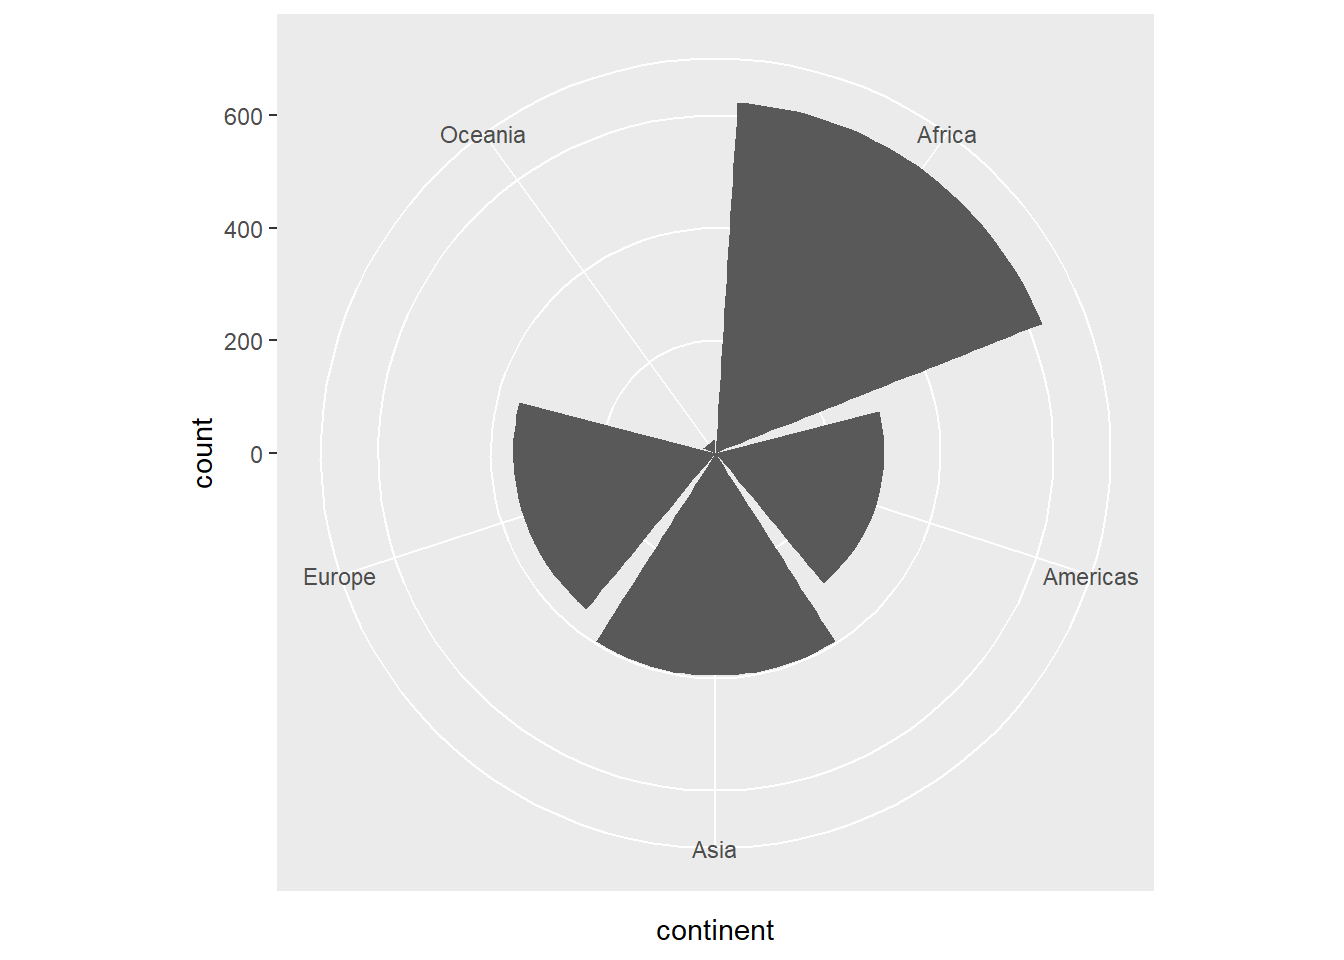
\includegraphics{bookdown-demo_files/figure-latex/unnamed-chunk-5-1.pdf}
If you would like to have a regular pie chart, then you need to provide the frequency distribution.

\hypertarget{histogram}{%
\section{Histogram}\label{histogram}}

\hypertarget{a-simple-histogram}{%
\subsection{A Simple Histogram}\label{a-simple-histogram}}

\begin{Shaded}
\begin{Highlighting}[]
\KeywordTok{library}\NormalTok{(ggplot2)}
\NormalTok{plot2 <-}\StringTok{ }\KeywordTok{ggplot}\NormalTok{(gapminder,}
                \KeywordTok{aes}\NormalTok{(}\DataTypeTok{x =}\NormalTok{ gdpPercap))}
\NormalTok{plot2 }\OperatorTok{+}\StringTok{ }\KeywordTok{geom_histogram}\NormalTok{(}\DataTypeTok{binwidth =} \DecValTok{1000}\NormalTok{)}
\end{Highlighting}
\end{Shaded}

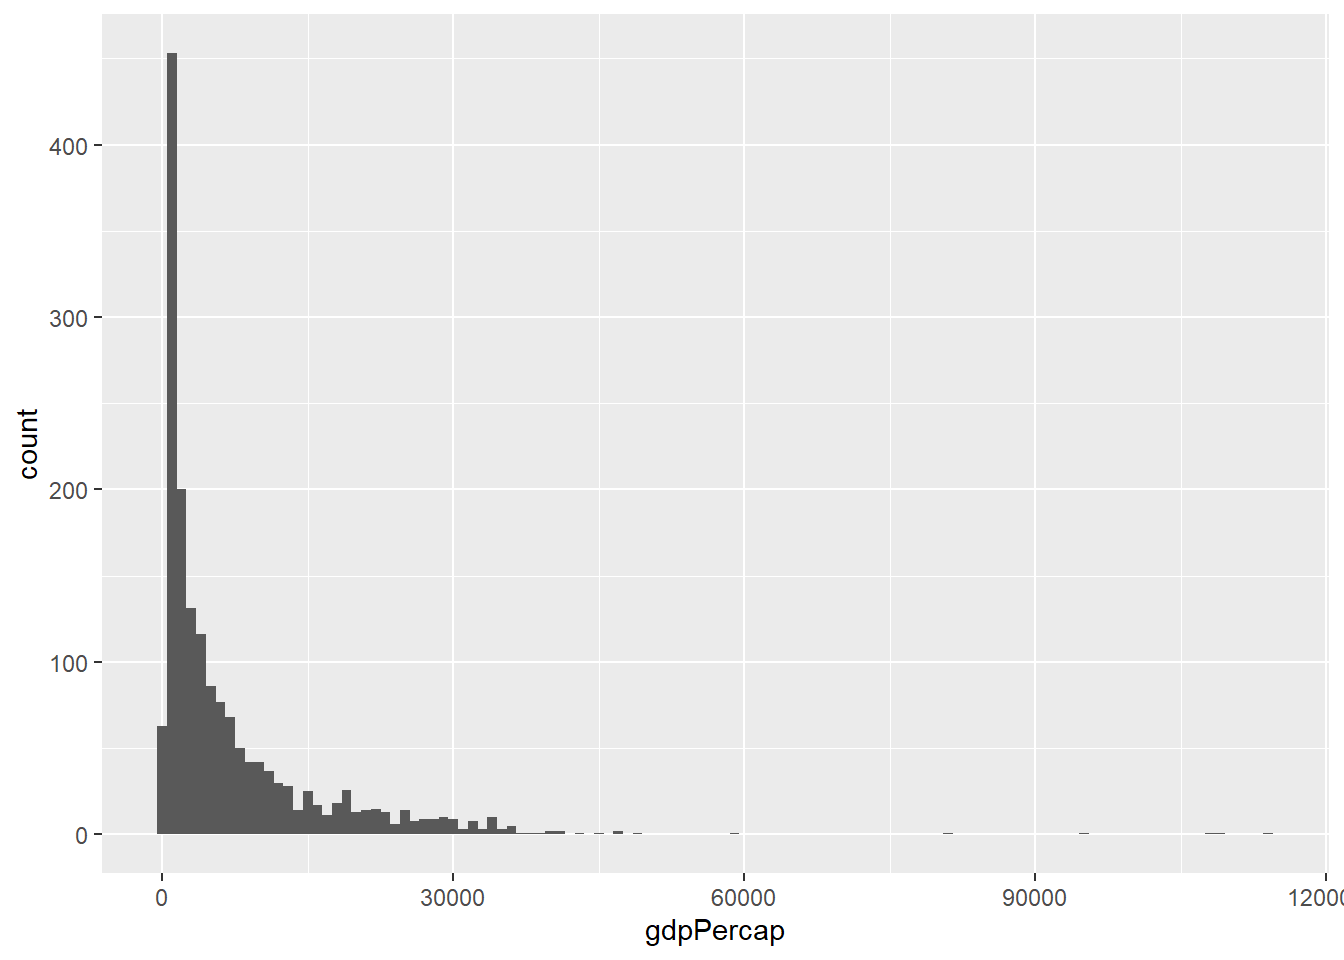
\includegraphics{bookdown-demo_files/figure-latex/unnamed-chunk-6-1.pdf}

\pagebreak

\hypertarget{histogram-with-a-title}{%
\subsection{Histogram With a Title}\label{histogram-with-a-title}}

\begin{Shaded}
\begin{Highlighting}[]
\NormalTok{plot2 }\OperatorTok{+}\StringTok{ }
\StringTok{  }\KeywordTok{geom_histogram}\NormalTok{(}\DataTypeTok{binwidth =} \DecValTok{1000}\NormalTok{) }\OperatorTok{+}
\StringTok{  }\KeywordTok{labs}\NormalTok{(}\DataTypeTok{title =} \StringTok{"Histogram of GDP per Capita for All Years"}\NormalTok{)}
\end{Highlighting}
\end{Shaded}

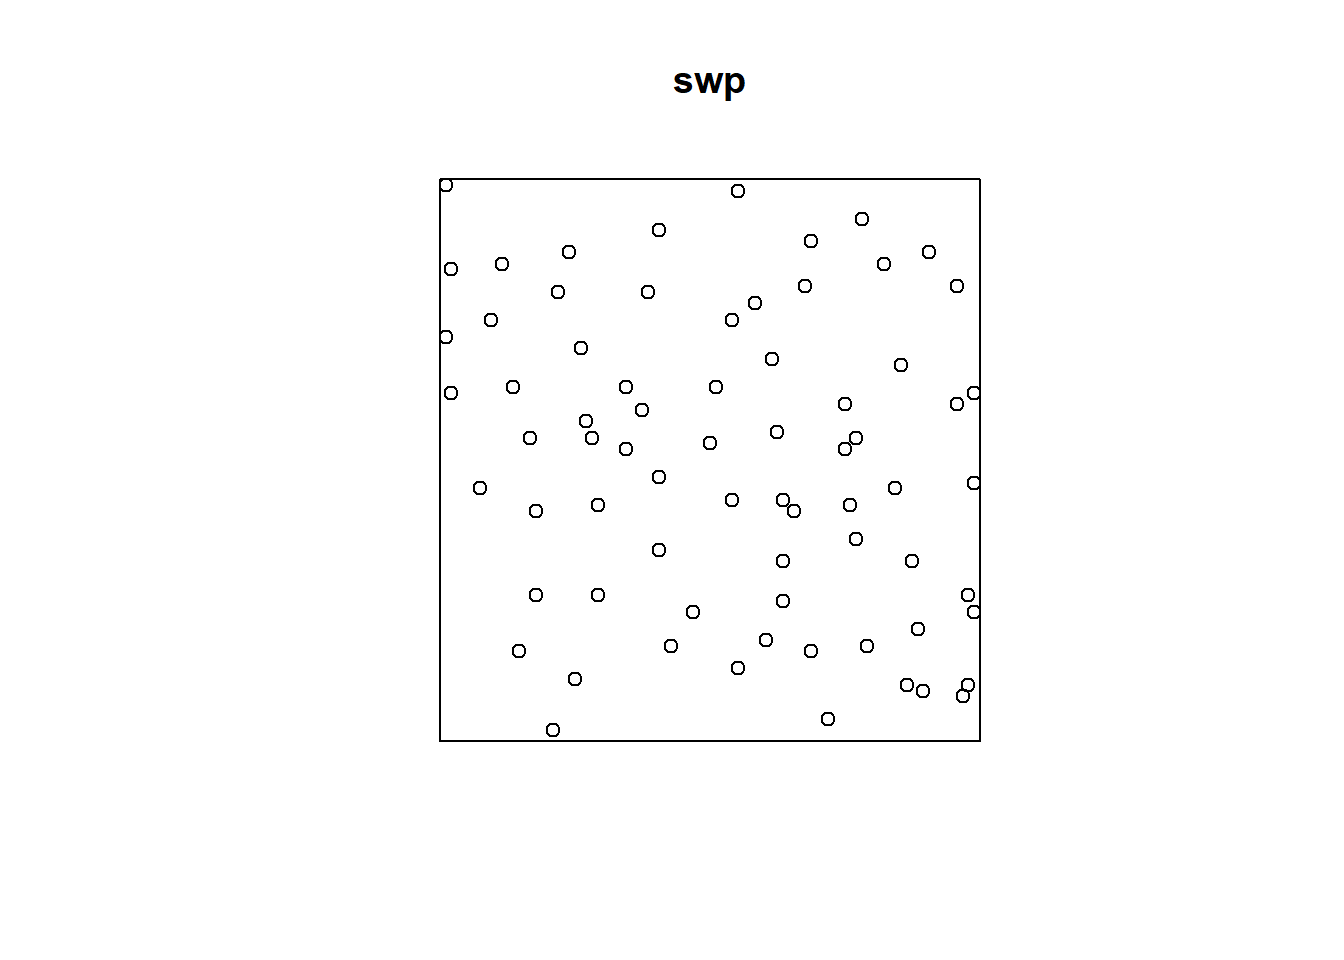
\includegraphics{bookdown-demo_files/figure-latex/unnamed-chunk-7-1.pdf}

\pagebreak

\hypertarget{histogram-with-different-color-schemes}{%
\subsection{Histogram with Different Color Schemes:}\label{histogram-with-different-color-schemes}}

\begin{Shaded}
\begin{Highlighting}[]
\NormalTok{plot2 }\OperatorTok{+}\StringTok{ }
\StringTok{  }\KeywordTok{geom_histogram}\NormalTok{(}\DataTypeTok{binwidth =} \DecValTok{1000}\NormalTok{, }\DataTypeTok{color=}\StringTok{"black"}\NormalTok{, }\DataTypeTok{fill=}\StringTok{"white"}\NormalTok{) }\OperatorTok{+}
\StringTok{  }\KeywordTok{labs}\NormalTok{(}\DataTypeTok{title =} \StringTok{"Histogram of GDP per Capita for All Years"}\NormalTok{)}
\end{Highlighting}
\end{Shaded}

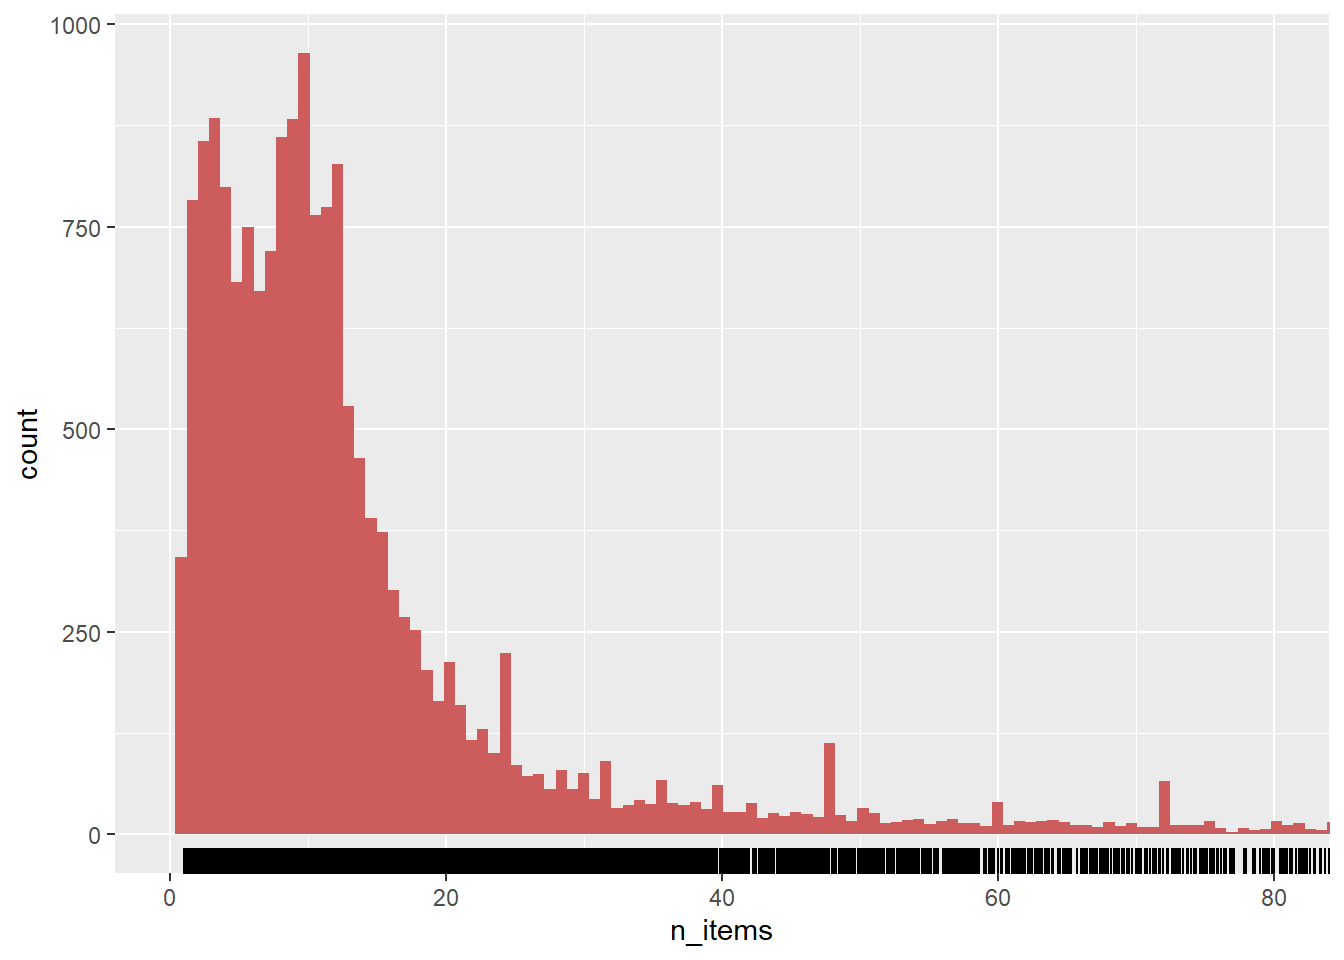
\includegraphics{bookdown-demo_files/figure-latex/unnamed-chunk-8-1.pdf}

\pagebreak

\hypertarget{histogram-of-log-transformed-variable}{%
\subsection{Histogram of Log Transformed Variable:}\label{histogram-of-log-transformed-variable}}

\begin{Shaded}
\begin{Highlighting}[]
\NormalTok{plot3 <-}\StringTok{ }\KeywordTok{ggplot}\NormalTok{(gapminder,}
                \KeywordTok{aes}\NormalTok{(}\DataTypeTok{x =} \KeywordTok{log10}\NormalTok{(gdpPercap)))}
\NormalTok{plot3 }\OperatorTok{+}\StringTok{ }
\StringTok{  }\KeywordTok{geom_histogram}\NormalTok{(}\DataTypeTok{binwidth =} \FloatTok{.2}\NormalTok{, }\DataTypeTok{color=}\StringTok{"black"}\NormalTok{, }\DataTypeTok{fill=}\StringTok{"white"}\NormalTok{) }\OperatorTok{+}
\StringTok{  }\KeywordTok{labs}\NormalTok{(}\DataTypeTok{title =} \StringTok{"Histogram of  Log Transformed GDP per Capita for All Years"}\NormalTok{)}
\end{Highlighting}
\end{Shaded}

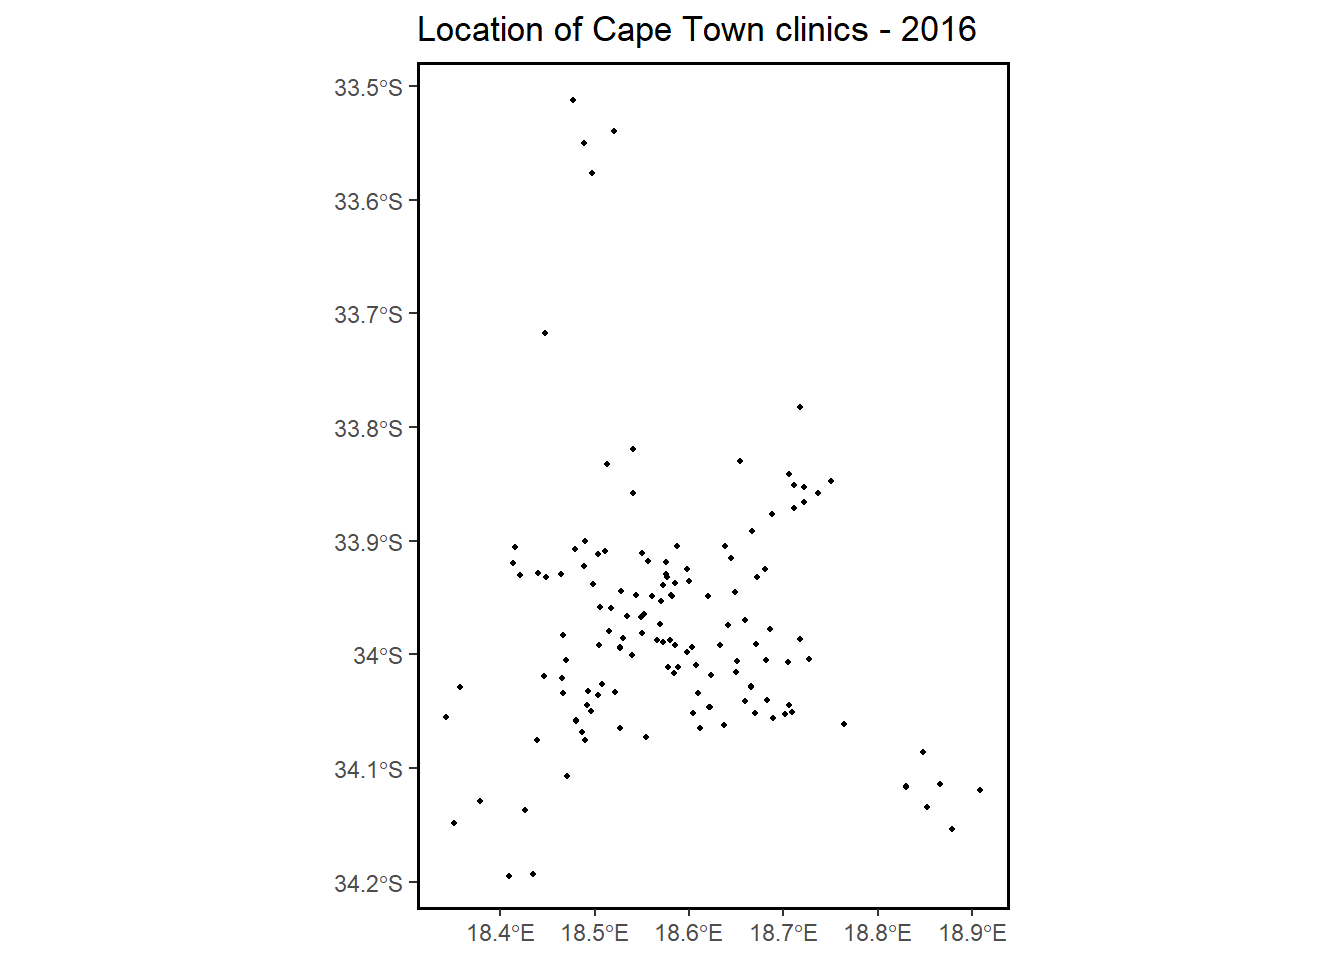
\includegraphics{bookdown-demo_files/figure-latex/unnamed-chunk-9-1.pdf}

\hypertarget{determine-the-binwidth}{%
\subsection{Determine the Binwidth}\label{determine-the-binwidth}}

How do we determine the binwidth?

\begin{itemize}
\item Sturges' rule uses class intervals of length \\
$L = \frac{x_{max}-x_{min}}{1+1.44*ln(n)}$ \\
\item Genstat rule uses uses class intervals of length: \\
$L = \frac{x_{max}-x_{min}}{\sqrt{n}}$ \\
\item or a general rule
\end{itemize}

So we can create our own function for the binwidth:

\begin{Shaded}
\begin{Highlighting}[]
\NormalTok{width_bin =}\StringTok{ }\ControlFlowTok{function}\NormalTok{(x) (}\KeywordTok{max}\NormalTok{(x)}\OperatorTok{-}\KeywordTok{min}\NormalTok{(x)) }\OperatorTok{/}\StringTok{ }\KeywordTok{sqrt}\NormalTok{(}\KeywordTok{length}\NormalTok{(x))}
\NormalTok{manualbin =}\StringTok{ }\KeywordTok{width_bin}\NormalTok{(}\KeywordTok{log10}\NormalTok{(gapminder}\OperatorTok{$}\NormalTok{gdpPercap))}
\end{Highlighting}
\end{Shaded}

\pagebreak

\begin{Shaded}
\begin{Highlighting}[]
\NormalTok{plot3 }\OperatorTok{+}\StringTok{ }
\StringTok{  }\KeywordTok{geom_histogram}\NormalTok{(}\DataTypeTok{binwidth =}\NormalTok{ manualbin, }\DataTypeTok{color=}\StringTok{"black"}\NormalTok{, }\DataTypeTok{fill=}\StringTok{"white"}\NormalTok{) }
\end{Highlighting}
\end{Shaded}

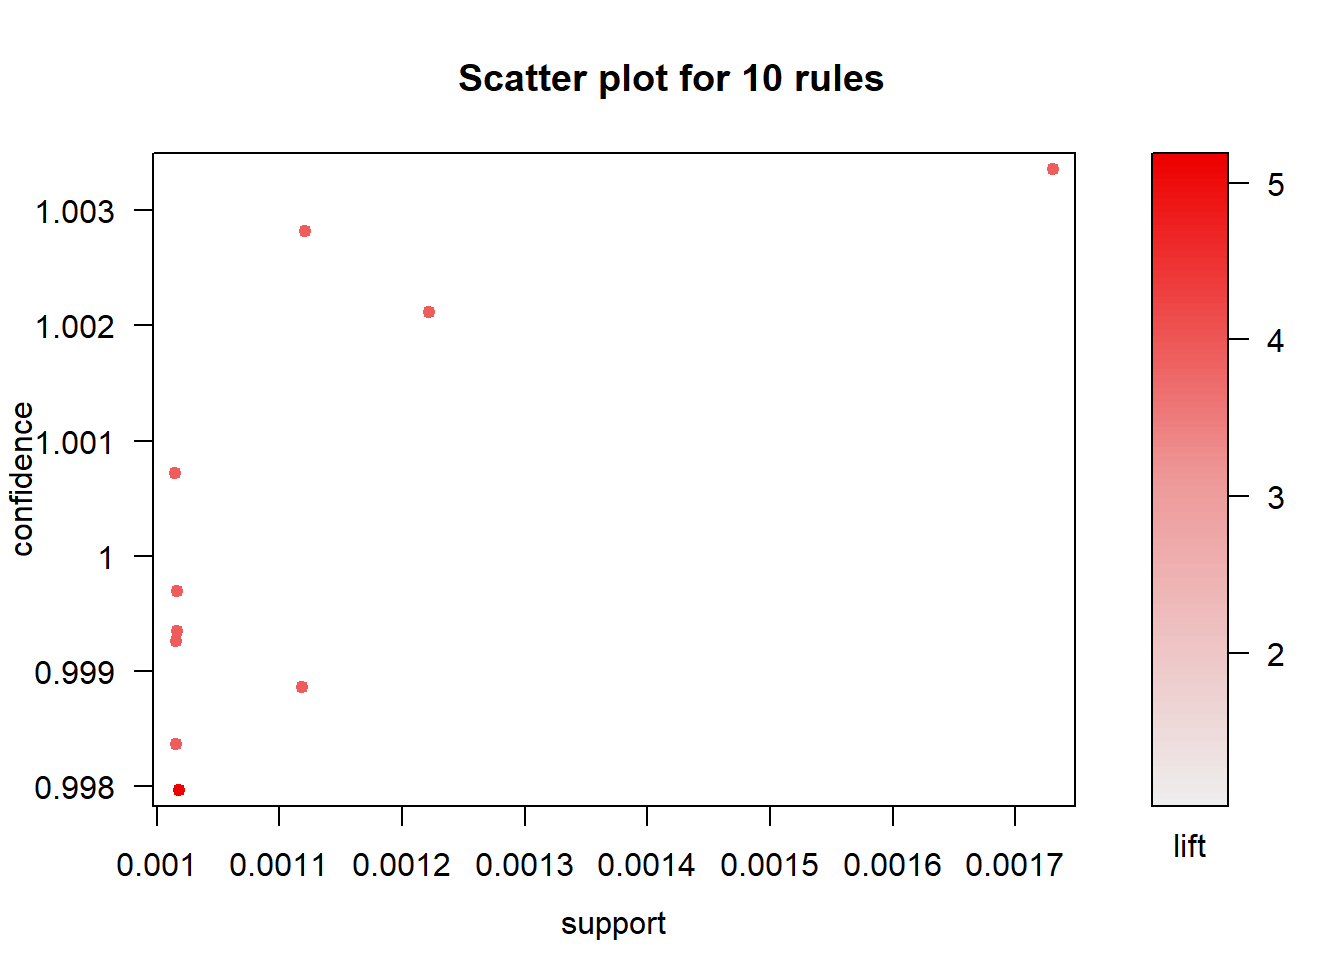
\includegraphics{bookdown-demo_files/figure-latex/unnamed-chunk-11-1.pdf}

\pagebreak

or simply

\begin{Shaded}
\begin{Highlighting}[]
\NormalTok{plot3 }\OperatorTok{+}\StringTok{ }
\StringTok{  }\KeywordTok{geom_histogram}\NormalTok{(}\DataTypeTok{binwidth =} \ControlFlowTok{function}\NormalTok{(x) (}\KeywordTok{max}\NormalTok{(x)}\OperatorTok{-}\KeywordTok{min}\NormalTok{(x)) }\OperatorTok{/}\StringTok{ }\KeywordTok{sqrt}\NormalTok{(}\KeywordTok{length}\NormalTok{(x)), }\DataTypeTok{color=}\StringTok{"black"}\NormalTok{, }\DataTypeTok{fill=}\StringTok{"white"}\NormalTok{) }\OperatorTok{+}
\StringTok{    }\KeywordTok{labs}\NormalTok{(}\DataTypeTok{title =} \StringTok{"Histogram of  Log Transformed GDP per Capita for All Years (Genstat Binwidth)"}\NormalTok{)}
\end{Highlighting}
\end{Shaded}

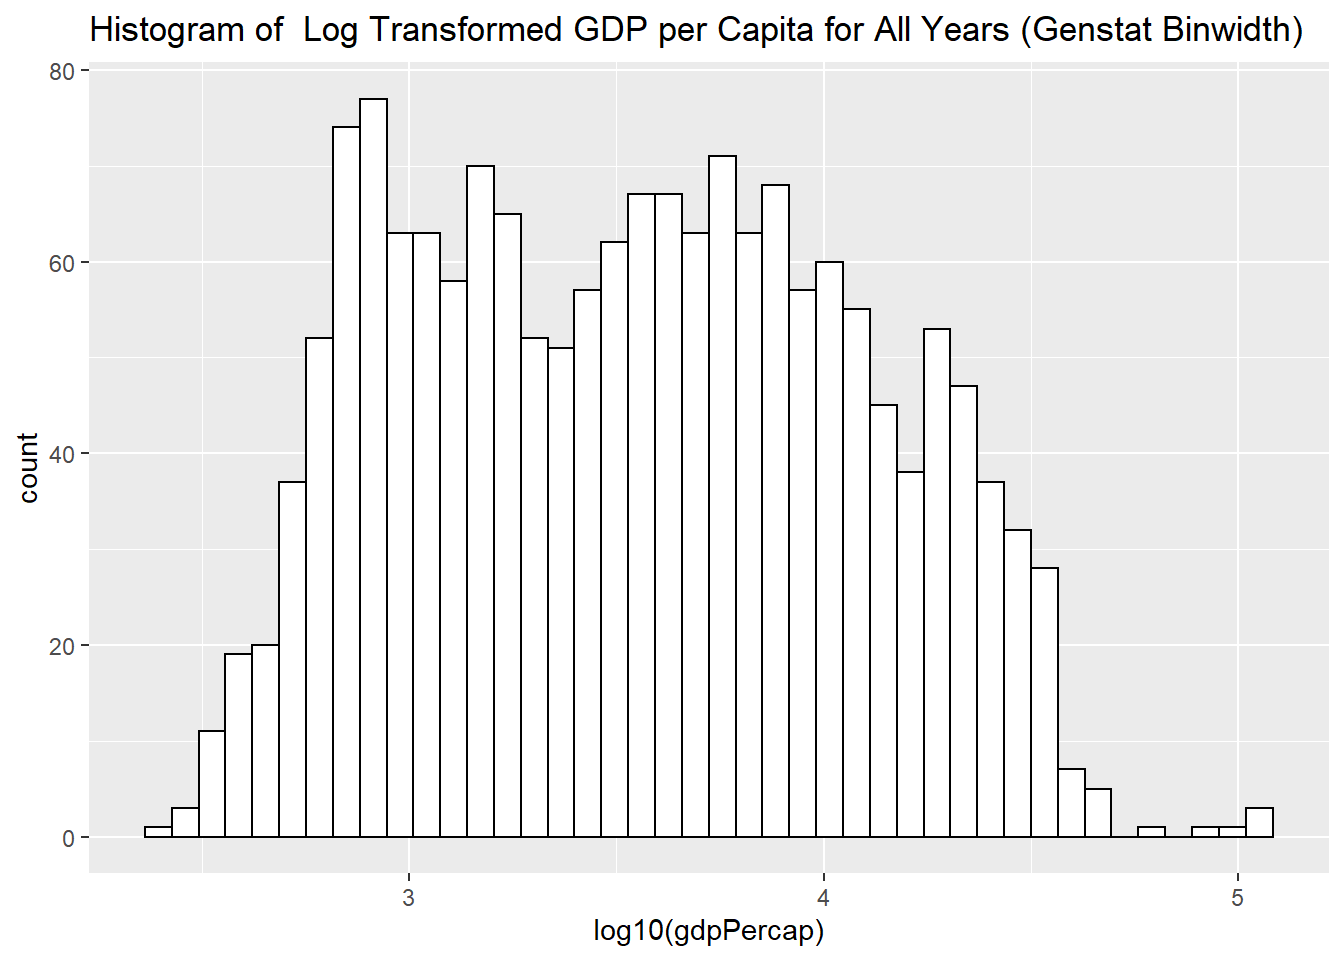
\includegraphics{bookdown-demo_files/figure-latex/unnamed-chunk-12-1.pdf}

But you will notice that Gdp per capita variable includes all years, all continents, all countries!!!

\pagebreak

\hypertarget{histogram-for-a-subset-of-data}{%
\subsection{Histogram for a Subset of Data}\label{histogram-for-a-subset-of-data}}

Log Transformed GDP per Capita for 2007:

\begin{Shaded}
\begin{Highlighting}[]
\NormalTok{plot4 <-}\StringTok{ }\KeywordTok{ggplot}\NormalTok{(}\KeywordTok{subset}\NormalTok{(gapminder, year }\OperatorTok{==}\StringTok{ }\DecValTok{2007}\NormalTok{),}
                \KeywordTok{aes}\NormalTok{(}\DataTypeTok{x =} \KeywordTok{log10}\NormalTok{(gdpPercap)))}
\NormalTok{plot4 }\OperatorTok{+}\StringTok{ }
\StringTok{   }\KeywordTok{geom_histogram}\NormalTok{(}\DataTypeTok{binwidth =} \ControlFlowTok{function}\NormalTok{(x) (}\KeywordTok{max}\NormalTok{(x)}\OperatorTok{-}\KeywordTok{min}\NormalTok{(x)) }\OperatorTok{/}\StringTok{ }\KeywordTok{sqrt}\NormalTok{(}\KeywordTok{length}\NormalTok{(x)), }\DataTypeTok{color=}\StringTok{"black"}\NormalTok{, }\DataTypeTok{fill=}\StringTok{"white"}\NormalTok{) }\OperatorTok{+}
\StringTok{  }\KeywordTok{labs}\NormalTok{(}\DataTypeTok{title =} \StringTok{"Histogram of  Log Transformed GDP per Capita for 2007 (Genstat Binwidth)"}\NormalTok{)}
\end{Highlighting}
\end{Shaded}

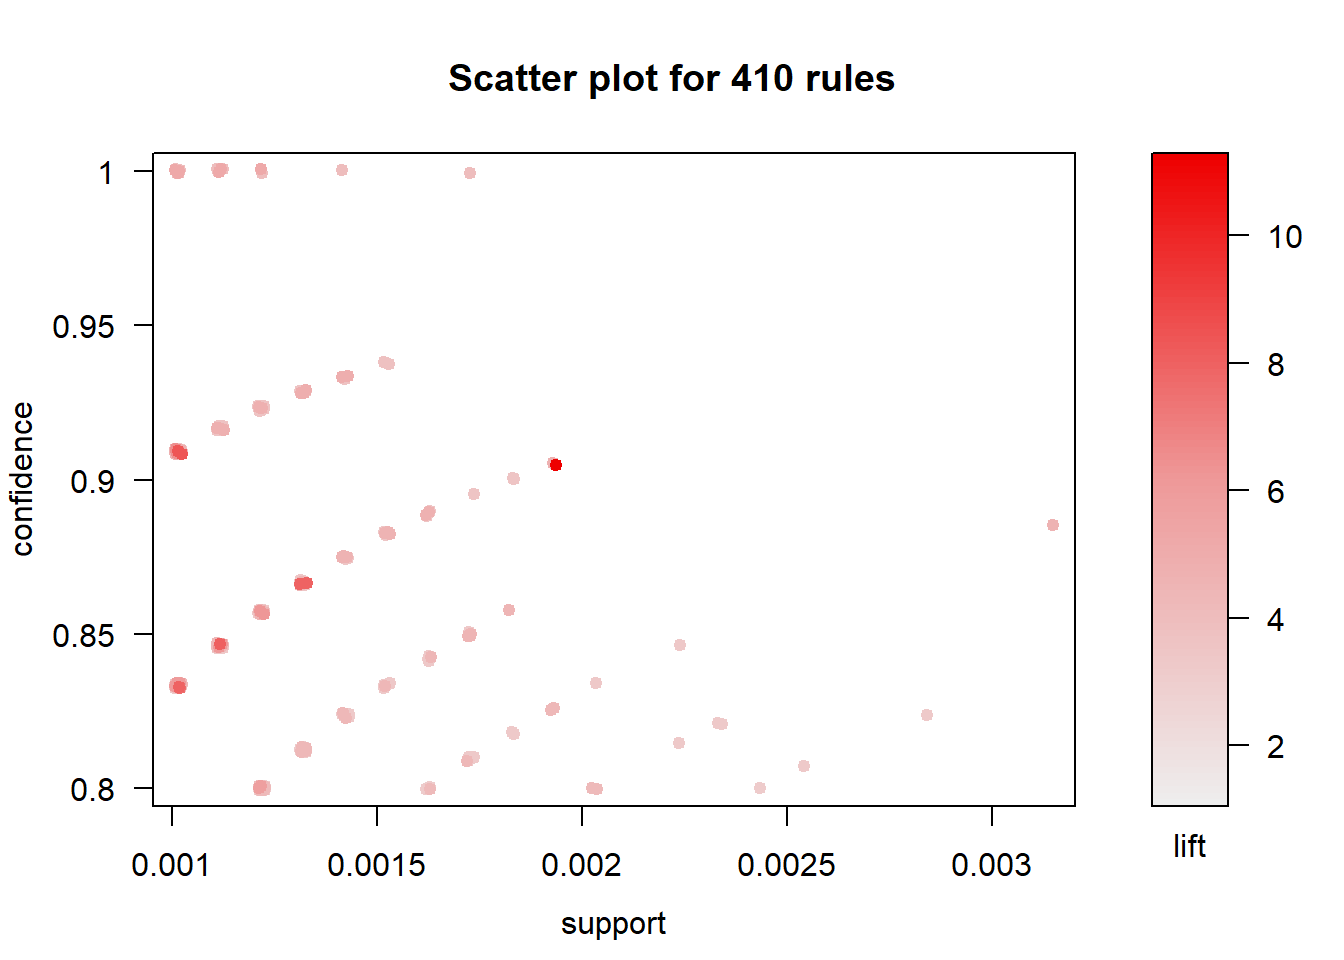
\includegraphics{bookdown-demo_files/figure-latex/unnamed-chunk-13-1.pdf}

\pagebreak

\hypertarget{histogram-with-overall-mean-line}{%
\subsection{Histogram with Overall Mean Line}\label{histogram-with-overall-mean-line}}

Log Transformed GDP per Capita for 2007 with the Overall Mean Line

\begin{Shaded}
\begin{Highlighting}[]
\CommentTok{# Histogram with mean of log10(gdpPercap) on the plot}
\NormalTok{plot4 }\OperatorTok{+}\StringTok{ }
\StringTok{  }\KeywordTok{geom_histogram}\NormalTok{(}\DataTypeTok{binwidth =} \ControlFlowTok{function}\NormalTok{(x) (}\KeywordTok{max}\NormalTok{(x)}\OperatorTok{-}\KeywordTok{min}\NormalTok{(x)) }\OperatorTok{/}\StringTok{ }\KeywordTok{sqrt}\NormalTok{(}\KeywordTok{length}\NormalTok{(x)), }\DataTypeTok{color=}\StringTok{"black"}\NormalTok{, }\DataTypeTok{fill=}\StringTok{"white"}\NormalTok{) }\OperatorTok{+}
\StringTok{  }\KeywordTok{geom_vline}\NormalTok{(}\KeywordTok{aes}\NormalTok{(}\DataTypeTok{xintercept=}\KeywordTok{mean}\NormalTok{(}\KeywordTok{log10}\NormalTok{(gdpPercap))),}
            \DataTypeTok{color=}\StringTok{"blue"}\NormalTok{, }\DataTypeTok{linetype=}\StringTok{"dashed"}\NormalTok{, }\DataTypeTok{size=}\DecValTok{1}\NormalTok{) }\OperatorTok{+}
\StringTok{  }\KeywordTok{labs}\NormalTok{(}\DataTypeTok{title =} \StringTok{"Histogram of  Log Transformed GDP per Capita for 2007 (Genstat Binwidth)"}\NormalTok{)}
\end{Highlighting}
\end{Shaded}

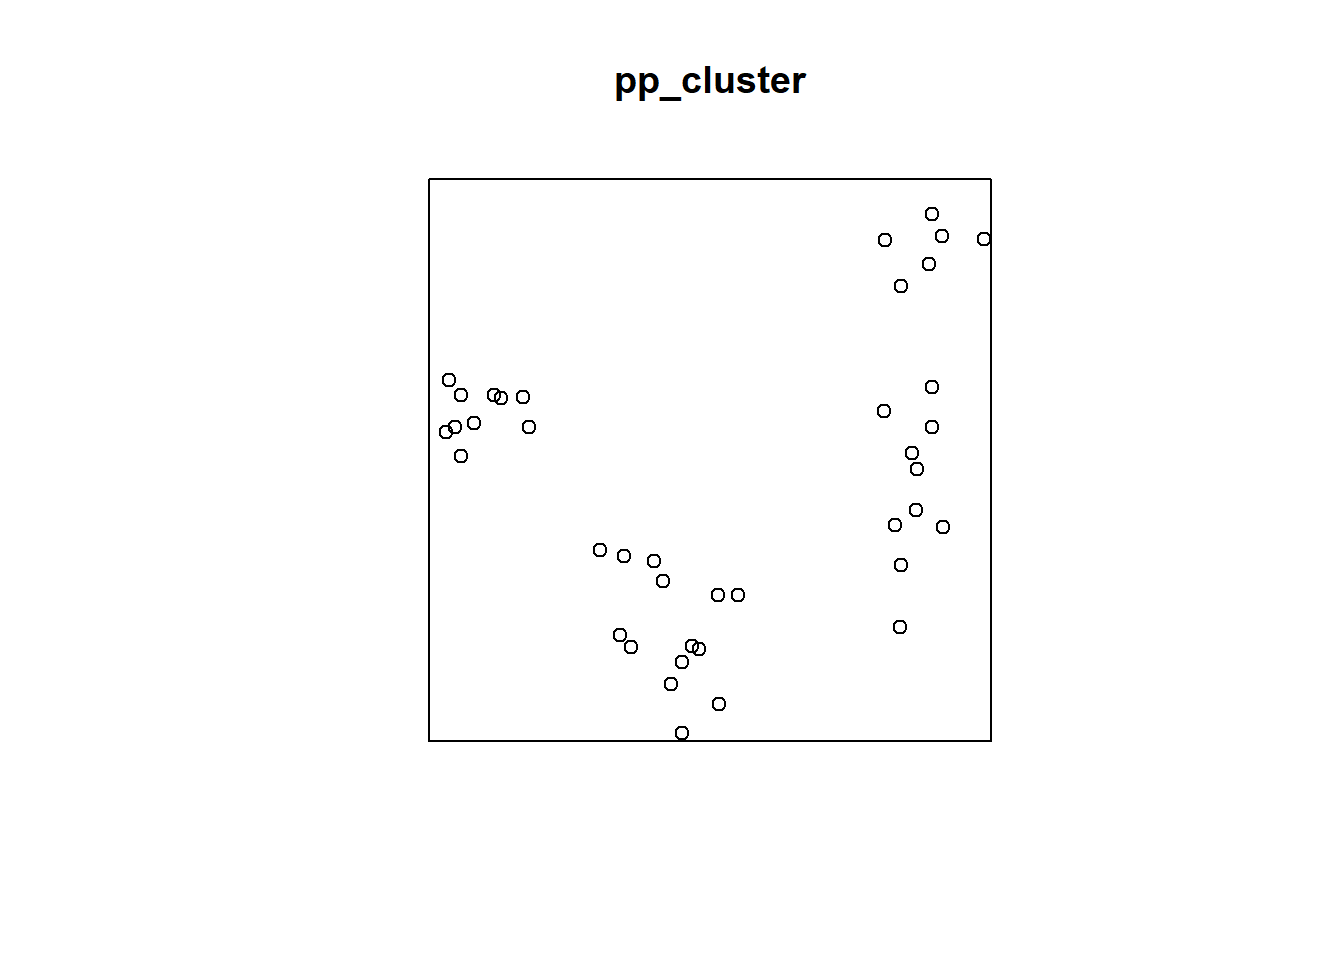
\includegraphics{bookdown-demo_files/figure-latex/unnamed-chunk-14-1.pdf}

\pagebreak

\hypertarget{histogram-with-density-plot}{%
\subsection{Histogram with Density plot}\label{histogram-with-density-plot}}

\begin{Shaded}
\begin{Highlighting}[]
\CommentTok{# Histogram with density plot}
\KeywordTok{ggplot}\NormalTok{(}\KeywordTok{subset}\NormalTok{(gapminder, year }\OperatorTok{==}\StringTok{ }\DecValTok{2007}\NormalTok{),}
                \KeywordTok{aes}\NormalTok{(}\DataTypeTok{x =} \KeywordTok{log10}\NormalTok{(gdpPercap))) }\OperatorTok{+}\StringTok{  }
\StringTok{  }\KeywordTok{geom_histogram}\NormalTok{(}\KeywordTok{aes}\NormalTok{(}\DataTypeTok{y=}\NormalTok{..density..), }\DataTypeTok{binwidth =} \ControlFlowTok{function}\NormalTok{(x) (}\KeywordTok{max}\NormalTok{(x)}\OperatorTok{-}\KeywordTok{min}\NormalTok{(x)) }\OperatorTok{/}\StringTok{ }\KeywordTok{sqrt}\NormalTok{(}\KeywordTok{length}\NormalTok{(x)),}\DataTypeTok{colour=}\StringTok{"black"}\NormalTok{, }\DataTypeTok{fill=}\StringTok{"white"}\NormalTok{)}\OperatorTok{+}
\StringTok{  }\KeywordTok{geom_density}\NormalTok{(}\DataTypeTok{alpha=}\DecValTok{0}\NormalTok{, }\DataTypeTok{fill=}\StringTok{"#FF6666"}\NormalTok{) }\CommentTok{#alpha for transparency, if alpha = 0, no fill}
\end{Highlighting}
\end{Shaded}

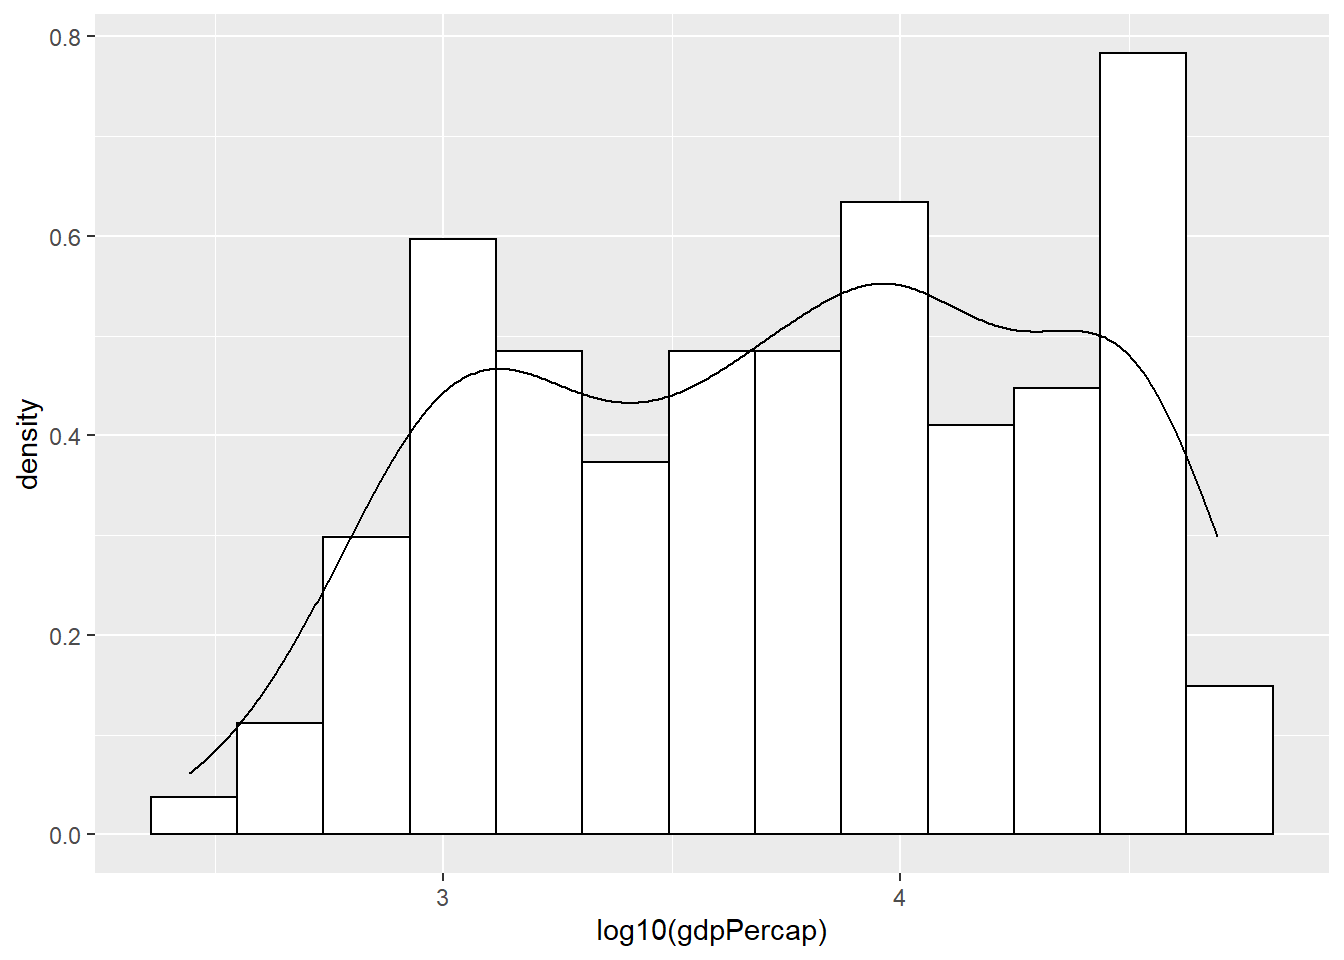
\includegraphics{bookdown-demo_files/figure-latex/unnamed-chunk-15-1.pdf}

\pagebreak

\hypertarget{histogram-with-facets}{%
\subsection{Histogram with Facets}\label{histogram-with-facets}}

How about looking at the differences among different continents?

\begin{Shaded}
\begin{Highlighting}[]
\CommentTok{# Histogram with mean of log10(gdpPercap) on the plot}
\NormalTok{plot4 }\OperatorTok{+}\StringTok{ }
\StringTok{  }\KeywordTok{geom_histogram}\NormalTok{(}\DataTypeTok{binwidth =} \ControlFlowTok{function}\NormalTok{(x) (}\KeywordTok{max}\NormalTok{(x)}\OperatorTok{-}\KeywordTok{min}\NormalTok{(x)) }\OperatorTok{/}\StringTok{ }\KeywordTok{sqrt}\NormalTok{(}\KeywordTok{length}\NormalTok{(x)), }\DataTypeTok{color=}\StringTok{"black"}\NormalTok{, }\DataTypeTok{fill=}\StringTok{"white"}\NormalTok{) }\OperatorTok{+}
\StringTok{  }\KeywordTok{geom_vline}\NormalTok{(}\KeywordTok{aes}\NormalTok{(}\DataTypeTok{xintercept=}\KeywordTok{mean}\NormalTok{(}\KeywordTok{log10}\NormalTok{(gdpPercap))),}
            \DataTypeTok{color=}\StringTok{"blue"}\NormalTok{, }\DataTypeTok{linetype=}\StringTok{"dashed"}\NormalTok{, }\DataTypeTok{size=}\DecValTok{1}\NormalTok{) }\OperatorTok{+}
\StringTok{  }\KeywordTok{facet_grid}\NormalTok{(continent }\OperatorTok{~}\StringTok{ }\NormalTok{.)}
\end{Highlighting}
\end{Shaded}

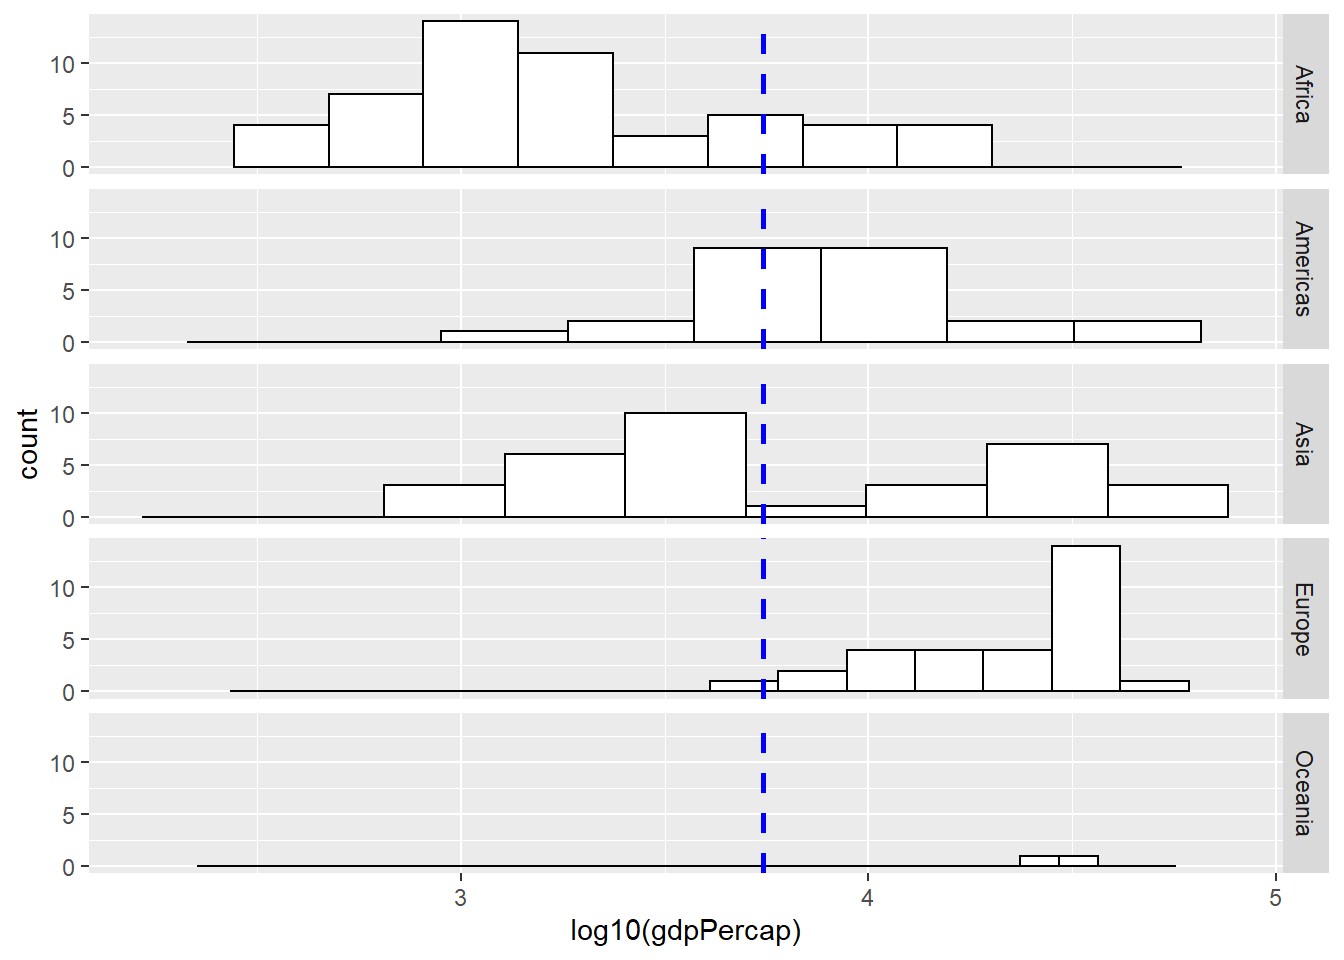
\includegraphics{bookdown-demo_files/figure-latex/unnamed-chunk-16-1.pdf}

\pagebreak

\hypertarget{boxplots}{%
\section{Boxplots}\label{boxplots}}

\begin{Shaded}
\begin{Highlighting}[]
\CommentTok{# Histogram with mean of log10(gdpPercap) on the plot}
\NormalTok{plot5 <-}\StringTok{ }\KeywordTok{ggplot}\NormalTok{(}\KeywordTok{subset}\NormalTok{(gapminder, year }\OperatorTok{==}\StringTok{ }\DecValTok{2007}\NormalTok{),}
                \KeywordTok{aes}\NormalTok{(}\DataTypeTok{x =}\NormalTok{ year, }\DataTypeTok{y =} \KeywordTok{log10}\NormalTok{(gdpPercap))) }
\CommentTok{# if x axis variable is numeric, then one single boxplot}
\CommentTok{# if x axis variable is categorical, then works like facets}

\NormalTok{plot5 }\OperatorTok{+}\StringTok{ }
\StringTok{  }\KeywordTok{geom_boxplot}\NormalTok{() }\CommentTok{#+ coord_flip()}
\end{Highlighting}
\end{Shaded}

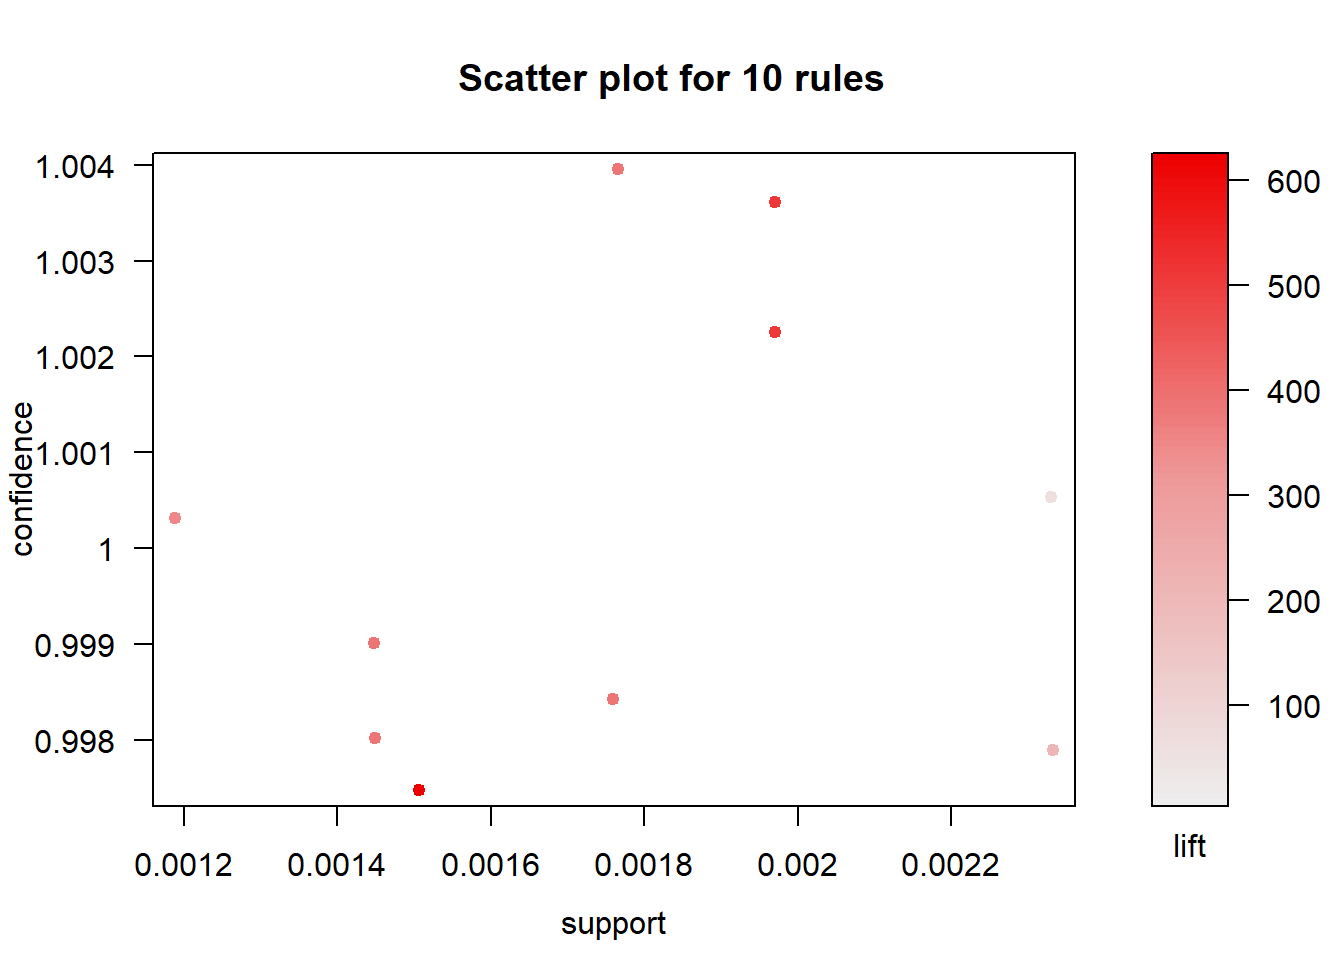
\includegraphics{bookdown-demo_files/figure-latex/unnamed-chunk-17-1.pdf}

Try with ``continent" variable.

\hypertarget{scatter-plots}{%
\section{Scatter Plots}\label{scatter-plots}}

\hypertarget{a-simple-scatter-plot}{%
\subsection{A Simple Scatter Plot}\label{a-simple-scatter-plot}}

\begin{Shaded}
\begin{Highlighting}[]
\NormalTok{plot6 <-}\StringTok{ }\KeywordTok{ggplot}\NormalTok{(}\KeywordTok{subset}\NormalTok{(gapminder, year }\OperatorTok{==}\StringTok{ }\DecValTok{2007}\NormalTok{),}
                \KeywordTok{aes}\NormalTok{(}\DataTypeTok{x =}\NormalTok{ lifeExp, }\DataTypeTok{y =} \KeywordTok{log10}\NormalTok{(gdpPercap)))}
\NormalTok{plot6 }\OperatorTok{+}
\StringTok{  }\KeywordTok{geom_point}\NormalTok{()}
\end{Highlighting}
\end{Shaded}

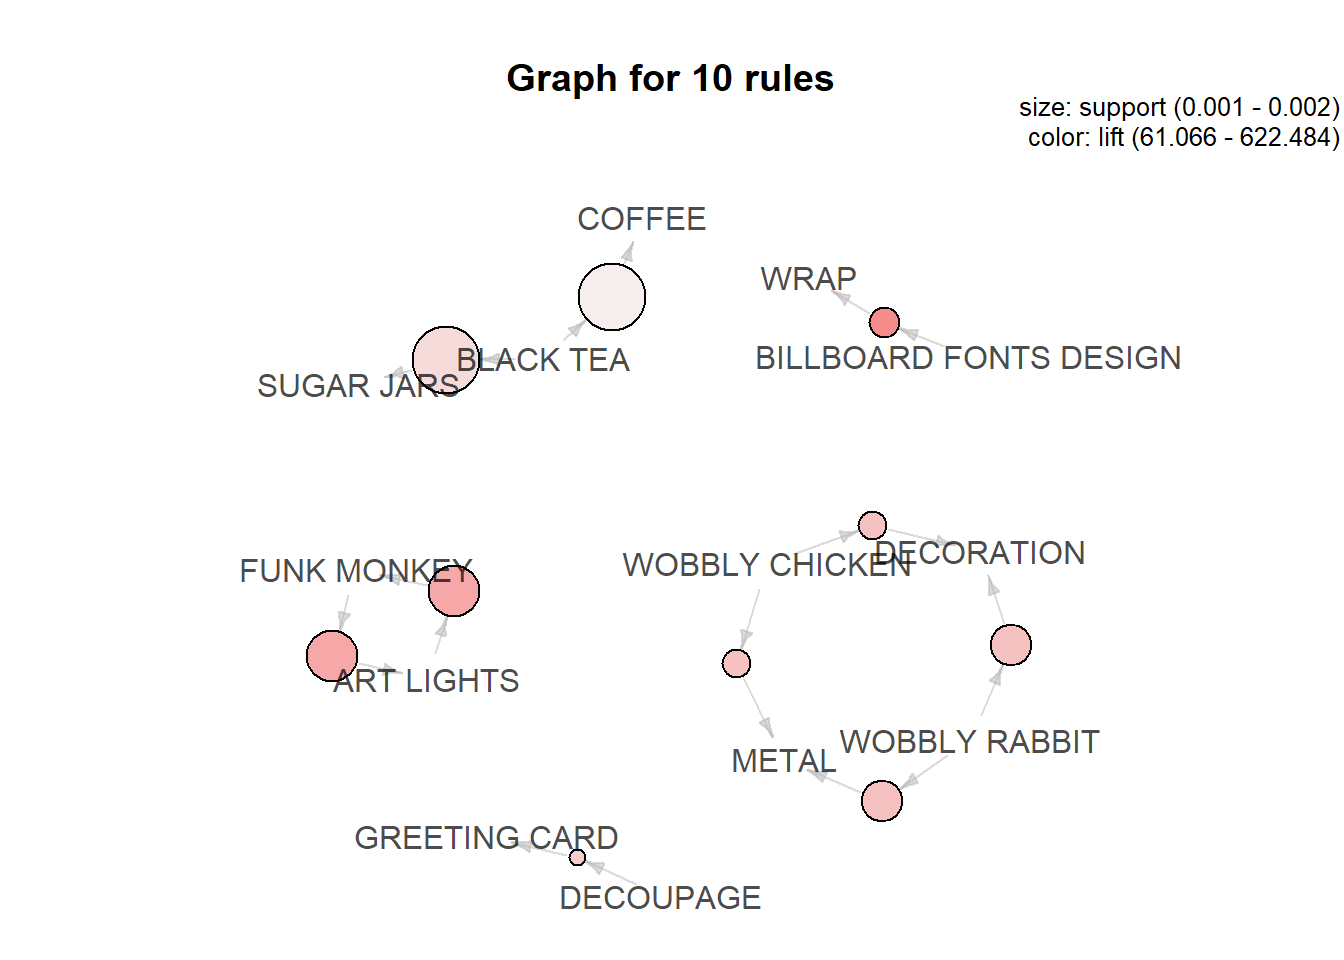
\includegraphics{bookdown-demo_files/figure-latex/unnamed-chunk-18-1.pdf}

\hypertarget{scatter-plot-with-labellings}{%
\subsection{Scatter Plot with Labellings}\label{scatter-plot-with-labellings}}

\begin{Shaded}
\begin{Highlighting}[]
\NormalTok{plot6 }\OperatorTok{+}
\StringTok{  }\KeywordTok{geom_point}\NormalTok{(}\KeywordTok{aes}\NormalTok{(}\DataTypeTok{colour =} \KeywordTok{factor}\NormalTok{(continent)))}
\end{Highlighting}
\end{Shaded}

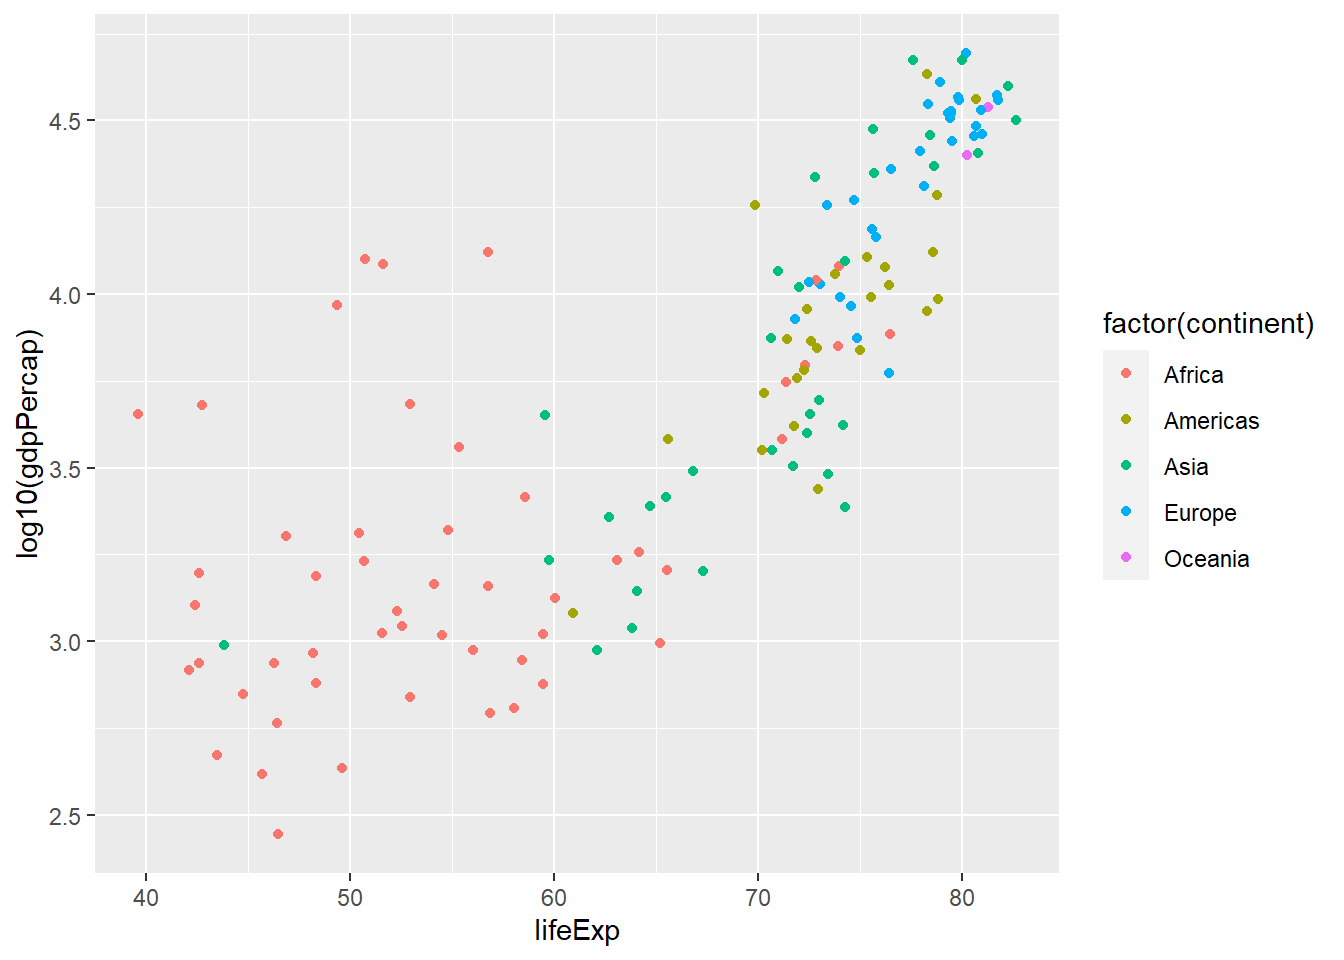
\includegraphics{bookdown-demo_files/figure-latex/unnamed-chunk-19-1.pdf}

\hypertarget{scatter-plot-with-linear-lines-for-different-groups}{%
\subsection{Scatter Plot with Linear Lines for Different Groups}\label{scatter-plot-with-linear-lines-for-different-groups}}

\begin{Shaded}
\begin{Highlighting}[]
\NormalTok{plot6 }\OperatorTok{+}
\StringTok{  }\KeywordTok{geom_point}\NormalTok{(}\KeywordTok{aes}\NormalTok{(}\DataTypeTok{colour =} \KeywordTok{factor}\NormalTok{(continent))) }\OperatorTok{+}
\StringTok{  }\KeywordTok{geom_smooth}\NormalTok{(}\KeywordTok{aes}\NormalTok{(}\DataTypeTok{group =}\NormalTok{ continent, }\DataTypeTok{colour =} \KeywordTok{factor}\NormalTok{(continent)), }\DataTypeTok{lwd =} \DecValTok{1}\NormalTok{, }\DataTypeTok{se =} \OtherTok{FALSE}\NormalTok{, }\DataTypeTok{method =} \StringTok{"lm"}\NormalTok{)}
\end{Highlighting}
\end{Shaded}

\begin{verbatim}
## `geom_smooth()` using formula 'y ~ x'
\end{verbatim}

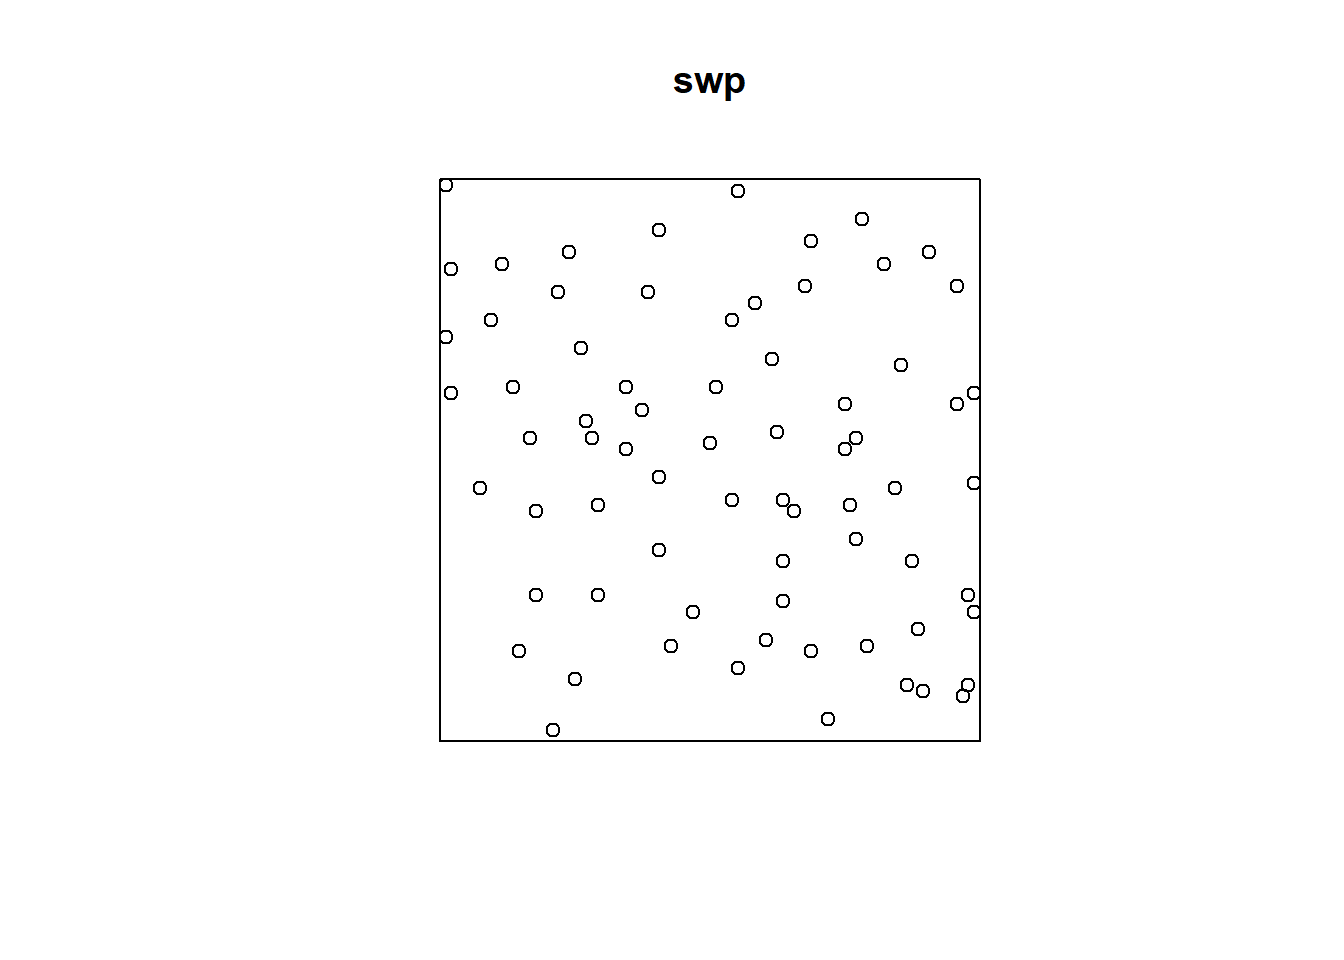
\includegraphics{bookdown-demo_files/figure-latex/unnamed-chunk-20-1.pdf}

\begin{Shaded}
\begin{Highlighting}[]
\NormalTok{plot7 <-}\StringTok{ }\KeywordTok{ggplot}\NormalTok{(gapminder,}
                \KeywordTok{aes}\NormalTok{(}\DataTypeTok{x =}\NormalTok{ lifeExp, }\DataTypeTok{y =} \KeywordTok{log10}\NormalTok{(gdpPercap)))}
\NormalTok{plot7 }\OperatorTok{+}
\StringTok{  }\KeywordTok{geom_point}\NormalTok{(}\KeywordTok{aes}\NormalTok{(}\DataTypeTok{colour =} \KeywordTok{factor}\NormalTok{(continent))) }\OperatorTok{+}
\StringTok{  }\KeywordTok{facet_wrap}\NormalTok{(}\OperatorTok{~}\StringTok{ }\NormalTok{year) }\CommentTok{# scales = "free_x"}
\end{Highlighting}
\end{Shaded}

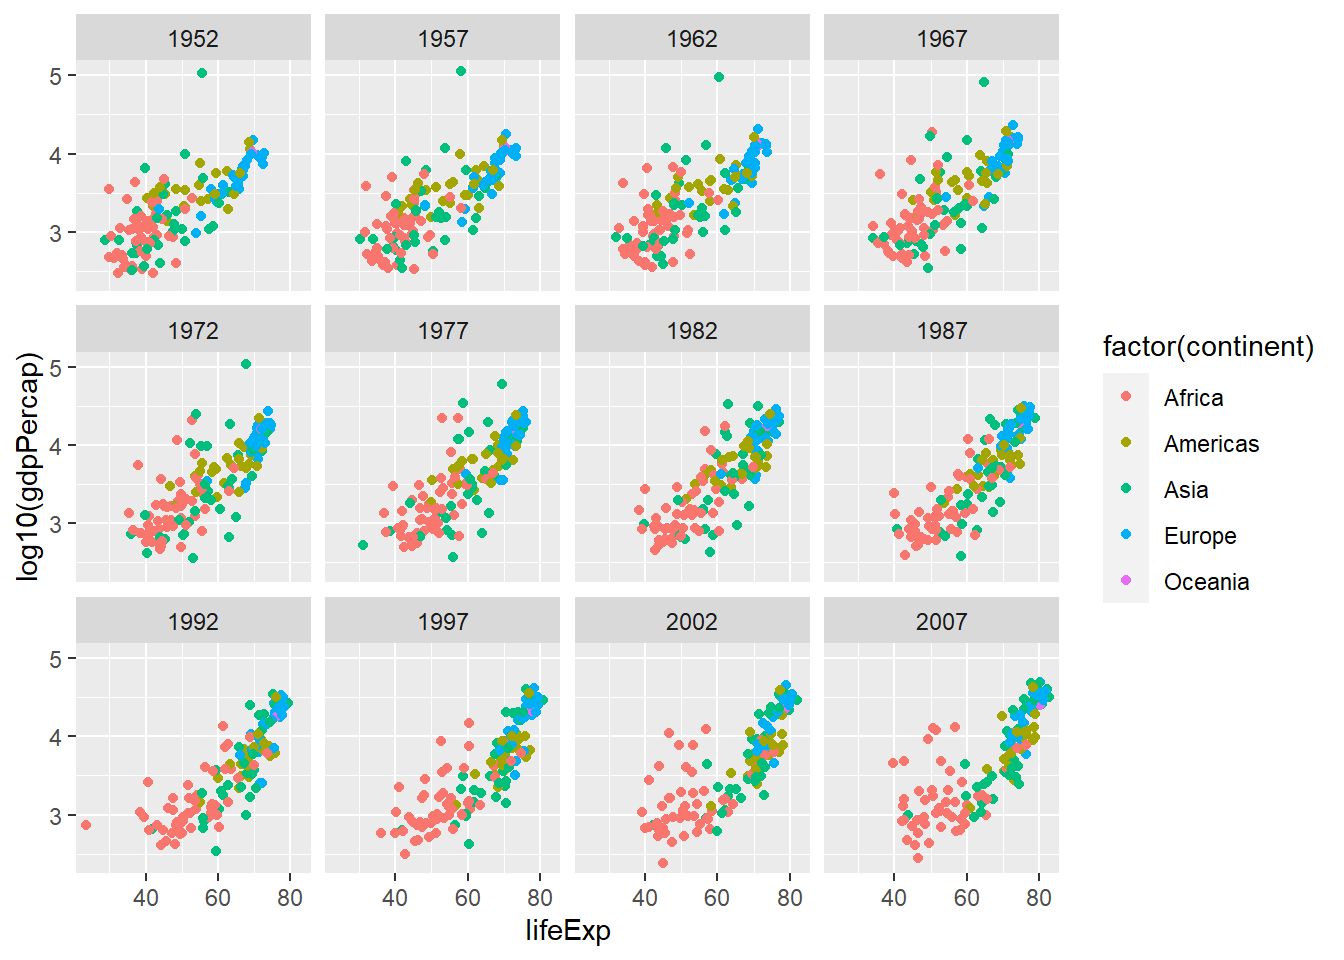
\includegraphics{bookdown-demo_files/figure-latex/unnamed-chunk-21-1.pdf}

For more check ``ggplot2: Elegant Graphics for Data Analysis (Use R!)" by (Hadley Wickham)

  \bibliography{book.bib,packages.bib}

\end{document}
